\documentclass[10pt,twocolumn,letterpaper]{article}

\usepackage{cvpr}
\usepackage{times}
\usepackage{epsfig}
\usepackage{graphicx}
\usepackage{amsmath}
\usepackage{amssymb}

% Include other packages here, before hyperref.

% If you comment hyperref and then uncomment it, you should delete
% egpaper.aux before re-running latex.  (Or just hit 'q' on the first latex
% run, let it finish, and you should be clear).
\usepackage[breaklinks=true,bookmarks=false]{hyperref}

\cvprfinalcopy % *** Uncomment this line for the final submission

\def\cvprPaperID{****} % *** Enter the CVPR Paper ID here
\def\httilde{\mbox{\tt\raisebox{-.5ex}{\symbol{126}}}}

% Pages are numbered in submission mode, and unnumbered in camera-ready
%\ifcvprfinal\pagestyle{empty}\fi
%\setcounter{page}{4321}
\begin{document}

\title{Applied Machine Learning Methodology Report}

\author{Moaz Mohamed\\
The University of Adelaide\\
Adelaide SA 5005\\
{\tt\small a1779177@student.adelaide.edu.au}
% For a paper whose authors are all at the same institution,
% omit the following lines up until the closing ``}''.
% Additional authors and addresses can be added with ``\and'',
% just like the second author.
% To save space, use either the email address or home page, not both
}

\maketitle
%\thispagestyle{empty}


%%%%%%%%% BODY TEXT
\section{Introduction}

There has been an increase of the usage of machine learning technique in medicine. from helping doctors predicting the severity of diseases \cite{Yao2020}, and using machine learning for protein folding problems \cite{Noe2020}. in this project machine learning will be used to re-purpose existing drugs to treat one of neglected tropical diseases visceral Leishmaniasis. Which is the most deadly species of the Leishmaniasis parasite. Drugs for Neglected Diseases initiative (DNDi) headquartered in Geneva, Switzerland has released the protien targets for Leishmaniasis parasite. an attempted will be made to use message passing neural network to predict the binding affinity \cite{Feinberg2018} of existing drugs at the market with the provided target protein from DNDi.

%-------------------------------------------------------------------------
\section{Chemical compounds representation}
The usage of machine learning in ligand based screening require having the lest amount reduction in information when representing a chemical compound. a popular representation method called Simplified molecular-input line-entry system (SMILES), its a one line notation encoding of a molecular structure. another representation is graphs. edges can have weights associated with how strong the bond is and each node can have a feature vector that can encode specific attributes for each node as each node represent a chemical element. whereas in SMILES only the elements and the bonds are encoded hence graphs is a better tool for representing chemical compounds \cite{Toropov2011}. 
%------------------------------------------------------------------------


\section{Deep Learning on Graphs}
\subsection{Graph Convolution Neural Network}

there are challenges on performing convolution operation on graphs due to the complex nature of graphs and the fact that with the different representation of graphs we can have different adjacency matrix hence the requirement of locality and aggregation of convolution isn't met \cite{Kipf2017}. 


\begin{figure}[h!]
  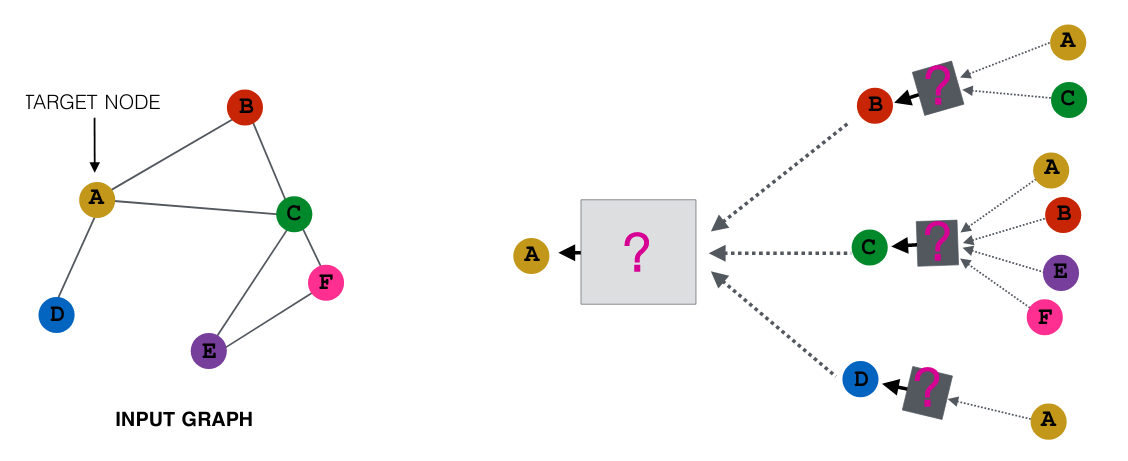
\includegraphics[width=\linewidth]{graph.png}
  \caption{graph computational model}
  \label{fig:graph}
\end{figure}


Different strategy is needed to apply different deep learning frameworks on graphs. In 2017 on " Neural Message Passing for Quantum Chemistry" \cite{Gilmer2017} outlines and summarized different machine learning methods to apply convolution or commonly what is known in graphs machine learning community as massage passing. the key idea is to use encoder like structure as having lower the dimentionality of a node. that is done by aggregating massages from the target node neighbors then applying a learn-able weight matrix and bias to encode the graph features into a lower dimension. by summing the feature vectors that are connected to the targeted node and multiplying it with a learn-able and differentiable wright matrix. its important to note that the summation operation is order invariant and the notion of depth instead of adding more layers as in typical neural network instead of Graph neural network we are borrowing information from more nodes or going deeper in the graph network to compute the summation and finally after applying the weight matrix and the activation function. we are left with a node embedding 


\begin{equation}
\mathbf{h}_{v}^{k}=\sigma\left(\mathbf{W}_{k} \sum_{u \in N(v)} \frac{\mathbf{h}_{u}^{k-1}}{|N(v)|}+\mathbf{B}_{k} \mathbf{h}_{v}^{k-1}\right)
\end{equation}

 

\subsection{Aggregation variants}

In GraphSage paper \cite{Hamilton2017}. instead of adding both the weight and the bias. the authors concatenated both terms and let the Back-propagation decide which term is more important ${W}_{k}$ or ${B}_{k}$, also the aggregation method isn't limited to finding the mean of the neighbors feature vectors. a pooling or applying a LSTM can be utilized and in the GraphSage paper using different aggregation resulted in better performance.  


\begin{equation}
\mathbf{h}_{v}^{k}=\sigma\left(\left[\mathbf{W}_{k} \cdot \operatorname{AGG}\left(\left\{\mathbf{h}_{u}^{k-1}, \forall u \in N(v)\right\}\right), \mathbf{B}_{k} \mathbf{h}_{v}^{k-1}\right]\right)
\end{equation}

\begin{equation}
\mathrm{AGG}=\gamma\left(\left\{\mathbf{Q h}_{u}^{k-1}, \forall u \in N(v)\right\}\right)
\end{equation}

\begin{equation}
\mathrm{AGG}=\mathrm{LSTM}\left(\left[\mathbf{h}_{u}^{k-1}, \forall u \in \pi(N(v))\right]\right)
\end{equation}


\section{Preparing data and loss function}

RDKit will be used to turn the smiles notation into graph representation and to generate the feature vectors for the edge. DeepChem will be used to provide atom feature vector. Since binding affinity is what is required for this project as a continuous prediction as a regression task the mean squared error will be used as a loss function.




{\small
\bibliographystyle{ieee_fullname}
\bibliography{MyCollection}
}

\end{document}
